\chapter{Wstęp}
\label{intro}

W~ramach pracy rozpatrywany jest problem weryfikacji postępów prac studentów dla przedmiotu, gdzie mamy zdefiniowane kilka grup projektowych.
Zadaniem każdego z~zespołów jest wykonanie, podczas trwania semestru, identycznego projektu.
Studenci przybliżają się do jego ukończenia poprzez zaliczanie kolejnych etapów.
Przykładem takiego przedmiotu są między innymi ”Podstawy Programowania”, prowadzone na wydziale Elektroniki i Technik Informacyjnych.

W pierwszym podrozdziale omówiono potrzebę oraz korzyści płynące z realizowania projektów grupowych w ramach programu studiów. 
Przedstawiony również został kierunek, w jakim będą zmierzać przedmioty projektowe w myśl reformy edukacji z roku 2018.

Kolejny podrozdział opisuje aktualny proces weryfikacji pracy studentów dla rozpatrywanych projektów grupowych.
Przybliżone są w nim problemy, na jakie napotykają prowadzący oraz studenci uczestniczący w tego typu przedmiocie.

W ramach podrozdziału \ref{programs-testing} przedstawiono ogólny trend co do potrzeby i nauki umiejętności testowania aplikacji przez studentów.
Omówiono także podstawowe rodzaje metod testowania: testowanie białej i czarnej skrzynki, wraz z wadami oraz zaletami tych podejść.

Ostatni podrozdział zawiera przegląd dostępnych, istniejących narzędzi wspomagających weryfikację umiejętności programistycznych użytkowników oraz ich zastosowanie.

\vfill

\section{Projekty grupowe}

Prowadzenie projektów grupowych niesie ze sobą wiele korzyści.
Na podstawie obserwacji obecnego rynku IT (ang. Information Technology) można stwierdzić, że większość komercyjnych projektów to projekty zespołowe.
Uczestnicząc w projekcie grupowym w ramach zajęć, student przystosowuje się do warunków, z jakimi zetknie się w swojej pierwszej pracy.

Projekt zespołowy pozwala na naukę pracy w grupie.
Wymusza na studentach komunikację zarówno z członkami zespołu, jak i z prowadzącym.
Kształtuje umiejętności analizy, właściwego podziału zadań oraz estymacji czasu ich wykonania.
Studenci uczą się również odpowiedzialności nie tylko za swoją pracę, ale również za efekty całego zespołu.
Niejednokrotnie biorą też udział w rozwiązywaniu konfliktów w grupie.
Wszystkie powyżej wymienione umiejętności są istotne podczas pracy zawodowej.


Umiejętność pracy w grupie jest bardzo pożądana przez pracodawców.
W ramach pracy [] zgrupowano i poddano ocenie miękkie umiejętności, jakimi powinni posługiwać się pracownicy branży IT.
Badania zostały przeprowadzone na podstawie analizy wymagań zawartych w 650 ofertach pracy z uwzględnieniem różnych lokalizacji.
Wyróżniono cztery kategorie stanowisk: analityków systemowych, projektantów oprogramowania, programistów oraz testerów.
Dla każdego ze stanowisk najwyżej cenione są umiejętności komunikacyjne.
Praca w grupie jest kolejną wskazywaną miękką umiejętnością.
Jest ona ceniona wyżej niż samodzielność w wykonywaniu zadań.
Zestawienie pożądanych umiejętności miękkich, jakimi powinni posługiwać się programiści, uzyskanych w ramach pracy F. Ahmed, L. F. Capretz, S. Bouktif i P. Campbell, zostało przedstawione na rysunku \ref{fig:soft-skills}.

\begin{figure}[h]
    \centering
    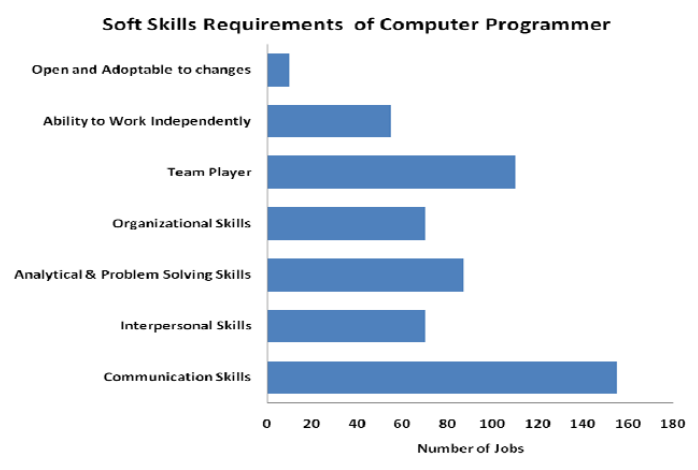
\includegraphics[width = 13cm]{chapter01/soft-skills.png}
    \caption{Pożądane umiejętności miękkie, jakimi powinni posługiwać się programiści (źródło []).}
    \label{fig:soft-skills}
\end{figure}

Również wśród pięciu podstawowych wartości, fundamentalnych dla Agile, wyróżnia się komunikację i szacunek [].
Jeśli przyjrzeć się bliżej definicjom podawanym między innymi przez Kent Beck [], obie te wartości można szlifować przez współpracę w ramach zespołu oraz współpracę z klientem (prowadzącym w przypadku studenckiego projektu grupowego).

Korzyści z projektów grupowych nie odnoszą się tylko do polepszenia umiejętności miękkich uczestników projektu.
Z założenia grupę projektową tworzą różne osoby, z których każda ma inne, własne zaplecze wiedzy technicznej.
Poprzez pracę w grupie studenci mają możliwość wymienienia się swoimi doświadczeniami i wiedzą.
Co więcej, mogą spojrzeć na ten sam zadany problem z różnych perspektyw i dojść do różnych wniosków.
Może to znacznie skrócić czas wykonania zadania i wyeliminować błędy na wczesnym etapie. 
Wymiana doświadczeń i dyskusje na temat różnych podejść do zadanego problemu mogą również rzutować na lepsze podejście do rozwiązywania zadań w przyszłości.

W myśl ustawy ”Prawo o szkolnictwie wyższym i nauce” z dnia 20 lipca 2018[], od semestru zima 2019, w ramach programu studiów będzie kładziony nacisk na prowadzenie projektów grupowych.
Jest to podyktowane dążeniem do zapewnienia wysokiej jakości kształcenia oraz właściwego przygotowania do wykonywania zawodu.

\vfill

\section{Proces weryfikacji pracy studentów}

Obecnie proces weryfikacji pracy studentów podczas semestru jest czasochłonny.
Każdy z prowadzących ma pod swoją opieką kilka (średnio od pięciu do siedmiu) grup projektowych.
W skład każdej grupy wchodzi około czterech studentów.
Projekt jest podzielony na kilka etapów. 
W przypadku przedmiotu podstawy programowania odbyło się sześć etapów zakończonych przesłaniem sprawozdania.

Poszczególne zadania wykonywane przez studentów są oceniane indywidualnie, pomimo powtarzalności zadań, jakie mają do wykonania zespoły.
W celu oceny pracy w ramach jednego etapu prowadzący przegląda kod zamieszczony przez studentów w systemie kontroli wersji, ocenia sprawozdanie oraz przeprowadza spotkanie ze studentami.
Przy ocenie postępów prowadzący bazuje na prezentacji programu wykonanej przez studentów lub na własnych doświadczeniach z interakcji z programem.

Przedstawienie prowadzącemu wyników cząstkowych oraz końcowych przez studentów może również okazać się kłopotliwe.
Manualne uruchamianie programów na prywatnych maszynach studentów jest czasochłonne.
Dodatkowo podczas przedstawiania wyników, mogą zaistnieć komplikacje związane między innymi z niepoprawną konfiguracją środowiska uruchomieniowego lub niewłaściwym doborem przypadków testowych.
W sytuacji, gdy zadaniem studentów jest zaprezentowanie interakcji pomiędzy stworzonymi przez nich modułami programów, prawdopodobieństwo wystąpienia powyższych błędów wzrasta.
Prowadzący, decydując się na samodzielne uruchomienie programów studentów, w celu ich oceny, jest również narażony na powyższe sytuacje.
W przypadku niedokładnej dokumentacji dotyczącej pracy studentów, jego zadanie może zostać znacznie utrudnione.
Taka sytuacja może doprowadzić do uzyskania niskiego wyniku przez studentów mimo niewielkich błędów w implementacji lub błędnie zrozumianych założeń.
Ze względu na indywidualne podejście do każdego z zespołów i etapów proces weryfikacji jest czasochłonny.

Studenci otrzymują informację dotyczącą oceny danego etapu, po jego zakończeniu.
W trakcie zadania oczywiście mogą doprecyzować szczegóły z prowadzącym.
Zdarza się jednak, że niektóre założenia są przez studentów zrozumiane w inny sposób niż oczekiwałby tego prowadzący.
W takim przypadku studenci podczas trwania etapu mogą napisać program zgodny z błędnie rozumianymi założeniami i dopiero po złożeniu etapu dowiedzieć się o niepoprawnej interpretacji zadania.
W obecnym procesie prowadzenia projektu informacja zwrotna dotycząca postępów pracy dociera do studentów stosunkowo późno.

Podczas prowadzenia projektu prowadzący napotykają również na problem braku systematycznej pracy studentów podczas semestru.
Może on wynikać częściowo z nie posiadania oficjalnej wiedzy o aktualnych postępach innych grup.
Podgląd statusu prac pozostałych zespołów mógłby być dodatkową motywacją dla studentów do wykonania danego etapu.

Proces prowadzenia projektów grupowych jest aktualnie usprawniany. 
Wśród tych usprawnień można wyróżnić między innymi zobligowanie studentów do zamieszczania
swojego kodu do systemu kontroli wersji. 
Jest to istotne usprawnienie, pozwalające na łatwiejsze przeglądanie kodu studentów i monitorowanie prac. 
Jednak studenci (zwłaszcza pierwszego roku) nie potrafią w pełni wykorzystać zalet tego narzędzia. 
Często nie zamieszczają kodu w postaci małych czytelnych commitów.
Zamiast tego zamieszczają całe paczki w formacie archiwalnym z nowymi wersjami oprogramowania.
Dokumentacja programów również nie jest zawsze pełna.
Dzięki wprowadzeniu systemu kontroli wersji prowadzący może przeglądać kod studentów na przystosowanym do tego interfejsie. 
Nie eliminuje to jednak czasochłonnego, indywidualnego podejścia do oceny każdej z grupy i etapów.




\section{Testowanie działania programu}
\label{programs-testing}

Dzięki wprowadzeniu systemu kontroli wersji można uzyskać szereg statystyk dotyczących pracy studentów.
Nie są to jednak pełne statystyki, które mogłyby interesować prowadzącego.
Sam kod zamieszczany w systemie, nie jest wystarczający do oceny etapu.
Co więcej, jego samodzielna analiza nie poprawiłaby a być może nawet pogorszyła czasochłonność weryfikacji wyników cząstkowych.
Ważnym elementem oceny poszczególnych etapów jest ocena poprawności działania uruchomionych programów dla zadanych danych testowych.

Można byłoby oczekiwać, że studenci sami pisaliby przypadki testowe dla swoich aplikacji. 
Podczas prezentacji ich zadaniem byłoby udowodnić, że testy kończą się pozytywnym wynikiem.
Niestety ciężko ocenić trafność napisanych przez studentów przypadków testowych.
Podjęcie się takiego zadania przez prowadzącego wymagałoby od niego jeszcze bardziej indywidualnego podejścia do grupy niż w przypadku sprawdzenia wyniku działania samego programu.
Jest to związane między innymi z tym, że część testów mogłaby się powtarzać, należałoby rozważyć priorytetyzajcę testowanych funkcjonalności, użyte narzędzia i poprawność asercji.
Takie zadanie mogłoby się okazać wyjątkowo ciężkie do zrealizowania w przypadku studentów, którzy są dopiero na początku swojej kariery programistycznej.
W takim przypadku studenci dopiero uczą się struktur języka i nie mają wystarczająco dużo wiedzy, aby napisać poprawnie testy [].

Na podstawie wyników ankiety portalu Stack Overflow z roku 2019 widać, że umiejętność testowania kodu jest bardzo istotna w przyszłej pracy [].
W ramach badania zapytano ankietowanych, czy w ich miejscach pracy używa się testów jednostkowych podczas wytwarzania oprogramowania.
Na rysunku \ref{fig:unit-tests-use} przedstawiono wyniki ankiety.
W przybliżeniu jeden na trzech ankietowanych nie używa testów najniższego poziomu w swoim procesie, ale zaledwie 4.4\% jest z tego zadowolona.
95.6\% osób testuje jednostkowo swoje aplikacje lub uważa, że ten rodzaj testów byłby przydatny w procesie wytwarzania oprogramowania. 
Warty uwagi jest również rezultat otrzymany w powiązaniu używania testów jednostkowych z poziomem satysfakcji z pracy ankietowanych, który został przedstawiony na rysunku \ref{fig:unit-tests-satisfaction}.
Osoby używające tego rodzaju testów są bardziej zadowolone ze swojej pracy.

\begin{figure}[h]
    \centering
    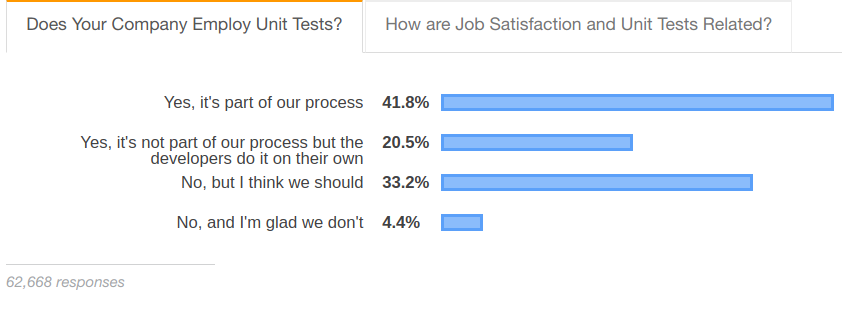
\includegraphics[width = 13cm]{chapter01/unit-tests-use.png}
    \caption{Używanie testów jednostkowych w procesie wytwarzania oprogramowania (źródło: []).}
    \label{fig:unit-tests-use}
\end{figure}

\begin{figure}[h]
    \centering
    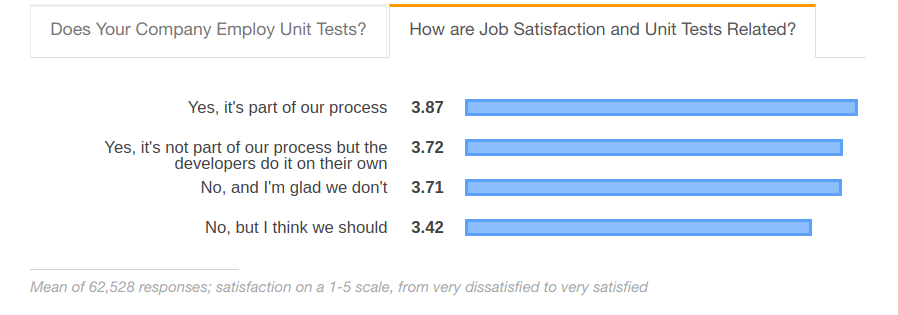
\includegraphics[width = 13cm]{chapter01/unit-tests-satisfaction.png}
    \caption{Powiązanie używania testów jednostkowych i zadowolenia z pracy (źródło: []).}
    \label{fig:unit-tests-satisfaction}
\end{figure}

Umiejętność testowania kodu jest często sprawdzana podczas procesu rekrutacyjnego.
Zarówno w przypadku, gdy kandydat ma za zadanie zaimplementować małe zdanie algorytmiczne, jak i napisać działającą aplikację.
W obu przypadkach musi on udowodnić poprawność swoje rozwiązania poprzez testy, niezależnie czy są to zaimplementowane testy wewnątrz aplikacji, czy poprzez analizę słowną przebiegu działania programu.
W pozycji pomagającej przygotować się do procesu rekrutacji ”Cracking the coding interview” [] testowaniu został poświęcony odrębny rozdział.

Programiści ćwiczący umiejętność testowania aplikacji potrafią lepiej wychwytywać potencjalne błędy na wczesnym etapie tworzenia oprogramowania [].
W przypadku małych i średnich firm wytwarzających oprogramowanie z wykorzystaniem podejścia Agile, często nie ma oddzielnych zespołów testerów.
W takich software house'ach zadaniem inżyniera oprogramowanie jest nie tylko napisanie działającej funkcjonalność, ale również samodzielne przetestowanie jej, poprzez testy jednostkowe i integracyjne.
W dużych korporacjach wykorzystujących metodyki Agile umiejętność testowania jest również istotna ze względu na ścisłą współpracę między interdyscyplinarnymi członkami zespołu.

Wśród pięciu wartości fundamentalnych dla zwinnego podejścia do wytwarzania oprogramowania jest wymieniona informacja zwrotna (ang. feedback) [].
Opisywana jest ona jako szybkość oceny poprawności dodawanego kodu oraz jego interakcji z innymi częściami systemu i ocenie regresji.
Szybką informację zwrotną dotyczącą dodawanej funkcjonalności można osiągnąć między innymi przez utrzymywanie poprawnych przypadków testowych.

Jedną z kategorii podziału testów, jest podział ze względu na wiedzę na temat testowanego programu.
W tym przypadku wyróżniamy dwie podstawowe kategorie:
\begin{itemize}
\item testy czarnej skrzynki (ang. black box testing),
\item testy białej skrzynki (ang. white box testing).
\end{itemize}

\begin{figure}[h]
    \centering
    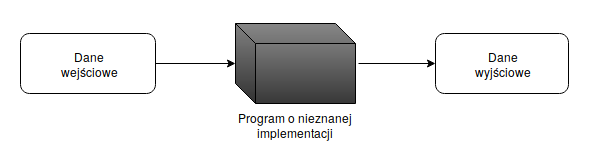
\includegraphics[width = 13cm]{chapter01/black-box.png}
    \caption{Schemat testu czarnej skrzynki (źródło własne).}
    \label{fig:black-box}
\end{figure}

Na rysunku \ref{fig:black-box} został przedstawiony ogólny schemat procesu dla black box testów.
Dla tego przypadku fragment kodu lub cały testowany program nie jest znany dla testera.
Black box testing może odnosić się zarówno do testów funkcjonalnych, jak i niefunkcjonalnych.
Najczęściej jednak dotyczy on pierwszego rodzaju.
Na rysunku \ref{fig:tests-levels} zostały przedstawione poziomy testów.
Testy czarnej skrzynki mają zastosowanie na następujących poziomach:
\begin{itemize}
\item testów integracyjnych,
\item testów systemowych,
\item testów akceptacyjnych.
\end{itemize}

\begin{figure}[h]
    \centering
    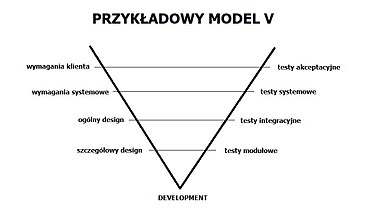
\includegraphics[width = 13cm]{chapter01/tests_levels.jpg}
    \caption{Poziomy testów (źródło własne).}
    \label{fig:tests-levels}
\end{figure}

Ten rodzaj testów jest wykonywany z perspektywy użytkownika.
Pozwala to między innymi na wskazanie rozbieżności pomiędzy wytworzonym kodem a założoną specyfikacją zadania w tym:
\begin {itemize}
\item niepoprawnych lub brakujących funkcjonalności,
\item błędów w interfejsie,
\item błędów w strukturach danych,
\item błędów zachowania programów oraz wydajnościowych.
\end{itemize}
Dodatkowo osoba testująca nie musi znać kodu oraz języka programowania, w którym została napisana aplikacja.

\begin{figure}[h]
    \centering
    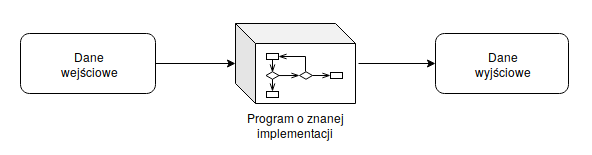
\includegraphics[width = 13cm]{chapter01/white-box.png}
    \caption{Schemat testu białej skrzynki (źródło własne).}
    \label{fig:white-box}
\end{figure}

Drugim rodzajem testowania programów jest metoda białej skrzynki (ang. white box testing).
Schemat procesu tego typu został przedstawiony na rysunku \ref{fig:white-box}.
W tym przypadku tester zna pełną implementację badanej funkcjonalności.
Jego zadaniem jest dobranie wartości wyjściowych dla sprawdzanej funkcjonalności i uzyskanie założonych wartości wyjściowych, w ramach testowanego kodu.
Do realizacji tego zadania niezbędne są umiejętności programistyczne i wiedza na temat implementacji.
Testy białej skrzynki mają zastosowanie na następujących poziomach:
\begin{itemize}
\item testów jednostkowych,
\item testów integracyjnych,
\item testów systemowych.
\end{itemize}
Warto jednak zaznaczyć, że ten typ testów używany jest głównie w testach jednostkowych.

Dzięki takiemu podejściu programiści mogą uzyskać bardzo szybką informację zwrotną.
Pozwala ono także na bardziej szczegółowe przetestowanie aplikacji.
Jednak poprawne napisanie testów jednostkowych jest bardziej złożone i wymaga dobrych umiejętności programistycznych.
Z założenia testów jednostkowych jest więcej niż integracyjnych czy akceptacyjnych i dla częstych zmian implementacji (co jest bardzo prawdopodobne na początkowym etapie nauki programowania) utrzymanie white box testów może okazać się bardzo kłopotliwe, a nawet wręcz niemożliwe dla studentów.
Warto też zauważyć, że testy jednostkowe są ściśle związane z implementacją, a więc z językiem programowania, w którym został napisany program.
W celu dodatnia testów najniższego poziomu należałoby posłużyć się dodatkową biblioteką, która byłaby wspomagana przez dany język.
Poznanie zewnętrznych bibliotek i zaznajamianie się z ich interfejsami na początkowej drodze nauki programowania mogłoby przynieść negatywne rezultaty.
Studenci, zamiast skupić się na zrozumieniu podstaw programowania, zmuszeni byliby do poznania bibliotek, dla których nie rozumieliby w pełni słuszności zastosowania.

W literaturze można znaleźć wiele prac poświęconych testowaniu programów i wprowadzaniu nauki umiejętności testowania w ramach programu studiów.
Kładziony jest coraz większy nacisk na tę umiejętność [].
Wśród zamieszczonych opinii powszechną jest, że testowanie aplikacji jest ważne i potrzebne od samego początku studiów [].
Wśród propozycji można znaleźć pomysł nauki pisania programów w metodyce TDD (ang. Test Driven Development) już od pierwszego semestru studiów [].
Wymagałoby to jednak wysokich kwalifikacji prowadzących co do znajomości metodyki i jej praktyki.
Warto zaznaczyć, że TDD opiera się na pisaniu testów jednostkowych, co, jak zostało wspomniane wcześniej, wymaga wiedzy na temat programowania.

Jak zostało napisane wcześniej, studentom rozpoczynającym naukę programowania bardzo ciężko byłoby napisać odpowiednie testy do swoich programów.
Praktycznie niemożliwe jest też wprowadzenie na początku studiów całego przedmiotu poświęconego nauce pisania testów, ze względu na przepełniony obecnie program studiów [].
Warto jednak pokazywać studentom zalety testowania aplikacji.
W przypadku jednakowych, wieloetapowych projektów prowadzący mógłby przygotować szereg przypadków testowych, które następnie zostałyby użyte do sprawdzenia poprawności programów studentów.
Idąc krok dalej, mógłby udostępnić je wcześniej studentom, aby mieli możliwość samodzielnie, lokalnie przetestować swój kod, przed ostateczną prezentacją prowadzącemu.
Taki proces sprawdzania programów studentów dla zadanych przypadków testowych można byłoby zautomatyzować tak, aby studenci mogli w prosty sposób wielokrotnie uruchamiać te same testy dla nowych wariantów swoich programów.
Opisany sposób testowania leży na poziomie testów akceptacyjnych w formie testów czarnej skrzynki.

Automatyzacja uruchamiania testów pozwoliłaby prowadzącemu na zmniejszenie czasochłonności oceny cząstkowych prac studentów.
Prowadzący mógłby oczekiwać, że programy, które pomyślnie przejdą przez testy akceptacyjne, są zaimplementowane prawidłowo.
Pozwoliłoby to na zniwelowanie indywidualnego podejścia do każdej z grupy.
Co więcej, studenci mogliby mieć wgląd do testów akceptacyjnych, dzięki czemu analizując przykłady, uczyliby się poprawnie definiować przypadki testowe.

W zależności od poziomu złożoności aplikacji wysokie pokrycie testowe mogłoby być jednak trudne do utrzymania.
Wraz ze wzrostem skomplikowania programów tworzenie przypadków testowych przez prowadzących stawałoby się coraz bardziej czasochłonne.

Ciekawym pomysłem zmniejszenia czasu jest zobligowanie studentów do samodzielnego pisania przypadków testowych, zebranie wszystkich testów i uruchomienie programu każdej grupy dla wszystkich zebranych przypadków. 
Słuszność takiego podejścia została opisana w artykule [].
Warto jednak zaznaczyć, że zadaniem prowadzącego w tym przypadku byłaby ocena jakości przypadków testowych.
Mogłoby się okazać, że zbiór testów ma stosunkowo niskie pokrycie, co jest wysoce prawdopodobne w przypadku studentów rozpoczynających naukę programowania.
Można jednak oczekiwać, że im większe doświadczenie studentów tym lepsze pokrycie aplikacji osiągniemy.

Innym pomysłem na zmniejszenie czasochłonności tworzenia testów akceptacyjnych jest porównywanie wyników programów studentów ze wzorcowym programem prowadzącego uruchomionym dla tych samych danych wejściowych.
W tym przypadku dane wejściowe mogłyby być generowane losowo.
Ten sposób chroniłby przed próbą implementacji programu, która generowałaby właściwy wynik tylko dla znanych wcześniej przypadków testowych.
To podejście ma też swoje wady, ponieważ używając zwykłego generatora losowego można uzyskać bardzo niskie pokrycie i nie przetestować poprawnie przypadków brzegowych.

Kolejnych innowacyjnym podejściem jest wykorzystanie metod ML (ang. Machine Learning) do generowania przypadków testowych. 
Ta metoda została opisana w pracy doktorskiej []. 
Dzięki uczeniu maszynowemu z wykorzystaniem prac studentów z poprzednich lat uzyskano narzędzie pozwalające generować przypadki testowe z bardzo wysokim pokryciem.
Trudno byłoby jednak zastosować podobną metodę do poprawienia procesu weryfikacji prac studentów, ze względu na brak dostępnych i dobrze opisanych programów studentów poprzednich lat.




\section{Narzędzia wspomagające ocenę umiejętności programistycznych}

Obecnie istnieje wiele narzędzi wspomagających ocenę umiejętności programistycznych użytkowników.
Są to najczęściej platformy z interfejsem webowych dostępne dla wszystkich.
Ogólna zasada działania tych narzędzi sprowadza się do napisania przez użytkownika prostego, odseparowanego programu z zadaną wejściową sygnaturą.
Następnie kod jest kompilowany, budowany i przepuszczany przez szereg testów akceptacyjnych.
Wynik testów jest przedstawiany użytkownikowi w postaci prostej wizualizacji.

Wśród narzędzi można wyróżnić strony umożliwiające testowanie umiejętności algorytmicznych użytkowników.
Pozwalają one zarówno na sprawdzenie poprawności wykonania implementowanych algorytmów, jak i oceny ich złożoności.
Wśród takich platform można wyróżnić między innymi: Codility [], HackerRank []. 
Pozwalają one także na przeprowadzanie zawodów w szybkim tworzeniu poprawnych i efektywnych algorytmów. 
Słuszność takich platform można potwierdzić między innymi na podstawie tego, że duże międzynarodowe korporacje takie jak Google zachęcają do przygotowywania się do procesów rekrutacyjnych z użyciem stron tego rodzaju. 
Niektóre mniejsze firmy prowadzą początkowe etapy rekrutacji z wykorzystaniem tych platform.

Innym rodzajem narzędzi są strony umożliwiające naukę programowania lub naukę programowania we wskazanym języku. 
Mogą być to proste symulatory środowisk, gdzie wraz z kolejnym etapem kursu użytkownik ma za zadanie napisać niewielki program lub jego część.
Czasem jednak narzędzia są bardziej rozbudowane i pozwalają na wizualizację działania programów w formie gry np. GameCoder [].
Podejście z tworzeniem gier jest wykorzystywane w celu zachęcenia i zainteresowania użytkowników oraz lepszego zobrazowania wyniku działania ich kodu.
Wśród narzędzi mających na celu lepsze zrozumienie wykonania kodu przez wizualizację można wyróżnić platformę do nauki programowania równoległego opisaną w artykule [].

W ramach pracy doktorskiej [] opisano narzędzie pozwalające na naukę pisania testów jednostkowych.
Bazując na danych historycznych, zaproponowano platformę pozwalającą na ocenę jakości testów pisanych przez użytkowników.
Jest to bardzo ciekawe i godne uwagi podejście do oceny umiejętności testowania programów przez studentów.

Narzędzia wspomagające ocenę umiejętności programistycznych są powszechne i mają różne zastosowania.
Skupiają się one jednak na niewielkich, pojedynczych, indywidualnych zadaniach.
Ze względu na powyższe cechy użycie ich w ramach wieloetapowego, długoterminowego i grupowego projektu nie jest wskazane.
W ramach pracy zaimplementowano i zbadano platformę umożliwiającą lepszą ocenę całego procesu tworzenia projektu z uwzględnieniem każdego etapu.
Proponowane rozwiązanie jest generyczne i poprzez odpowiednie zdefiniowanie środowiska uruchomieniowego może zostać użyte dla dowolnego języka programowania.




\section{Platforma testowa - założenia}

W ramach pracy zaproponowano i zaimplementowano platformę wspomagającą weryfikację pracy studentów podczas projektu grupowego. 
Omawiane narzędzie zostało utworzone jako MVP (ang. Minimal Value Product). 
Oznacza to, że podczas implementacji ograniczono się do dodania głównych funkcjonalności, pozwalających na wykorzystanie narzędzia podczas prowadzenia przedmiotu realizującego projekt grupowy.
Pozostałe, dodatkowe funkcjonalności mogą zostać dodane w ramach rozwinięcia pracy.

Podstawowym zadaniem platformy jest zredukowanie czasochłonności procesu weryfikacji pracy studentów wynikającej z indywidualnego podejścia przy rozpatrywaniu cząstkowych rezultatów dla każdej z grup.
To założenie można osiągnąć poprzez automatyzację procesu sprawdzania wyników wykonania programów w ramach kolejnych etapów.
Automatyzacja sprowadzałaby się do utworzenia szeregu przypadków testowych przez prowadzącego w ramach każdego z etapów.
Następnie programy napisane przez studentów, zostałyby przepuszczane przez testy akceptacyjne.
Wynik testów byłby znany zarówno dla prowadzącego, jak i studentów.
Otrzymane rezultaty byłby jednoznaczne.
Jeśli wszystkie testy zakończyłyby się sukcesem, to dana grupa zaliczyłaby w pełni zadany etap.
W przypadku, gdy któryś z testów ukończyłby się błędem, aplikacja studencka nie spełniałaby wszystkich założeń projektowych.
Na podstawie znajomości ilości i rodzaju testów, które zakończyły się niepoprawnie, prowadzący miałby jasną sytuację co do postępów pracy dla zadanego etapu.
Te same testy służyłyby do weryfikacji cząstkowej pracy każdej z grup, dzięki czemu prowadzący nie musiałby już indywidualnie oceniać poprawności programów.

Wymuszenie usunięcia indywidualnego podejścia do grup nie jest w pełni możliwe. 
Obecnie w ramach każdego etapu studenci udostępniają swoje sprawozdania z postępów prac prowadzącym.
Analiza i ocena dokumentów musi odbyć się indywidualnie dla każdej grupy.
Studenci zamieszczają sprawozdania korzystając z systemu kontroli wersji.
Dokumenty jednak nie zawsze znajdują się w jasno określonym, intuicyjnym miejscu w repozytorium, a odnalezienie ich zajmuje zbędny czas.
Również w przypadku kodu programu niejednokrotnie ciężko stwierdzić, która wersja jest ostateczna dla zadanego etapu.
W celu ułatwienia oceny pracy studentów należałoby zebrać w jednym, intuicyjnym miejscu trzy elementy cząstkowej pracy studentów pozwalające na jej ocenę: program wykonywalny, link do kodu aplikacji oraz sprawozdanie.
Dzięki łatwemu dostępowi do tych elementów prowadzący może uniknąć błędów podczas oceniania etapu.
 
Aktualnie informacja zwrotna dotycząca wyniku uzyskanego dla zadanego podzadania jest przekazywana studentom na zakończenie etapu.
Jest to stosunkowo późny moment.
Uzyskanie informacji zwrotnej przez grupę można przyspieszyć, poprzez udostępnienie im narzędzia pozwalającego na wielokrotne sprawdzenie działania programu przy użyciu zdefiniowanych przez prowadzących testów akceptacyjnych.
Umożliwiając studentom samodzielne sprawdzenie ich aplikacji, pozwalamy im na zdobycie w szybszym czasie informacji o nieprawidłowościach w ich programie.
Dzięki temu studenci mają czas na eliminację błędów i doprecyzowanie założeń na wstępnym etapie implementacji danego etapu.
Studenci powinni mieć wgląd do pełnej definicji wszystkich przypadków testowych, aby mogli lepiej zrozumieć błędne działanie swoich aplikacji.
Wśród informacji zwrotnej dla każdego z testów powinny znajdować się:
\begin{itemize}
\item dane wejściowe,
\item oczekiwane dane wyjściowe oraz zwrócony wynik,
\item status,
\item logi aplikacji.
\end{itemize}

Zadaniem grupy studentów korzystającego z platformy jest zamieszenie na niej wyników swojej pracy dla kolejnych etapów.
Należą do nich: sprawozdanie, link do kodu oraz program.
Platforma powinna umożliwiać umieszczanie dokumentu w dowolnym formacie.
Użytkownicy powinny móc w intuicyjny sposób przejść do kodu programu powstałego dla zadanego etapu poprzez link prowadzący do odpowiedniego commita w systemie kontroli wersji.
W wersji MVP kod studentów nie zakłada się kompilacji kodu na platformie.
Oczekuje się, że studenci sami zbudują swoje projekty i zamieszczą na platformie wykonywalne programy.
Warto zaznaczyć, że umieszczane aplikacje mogą zawierać istotne błędy powodujące przykładowo wycieki pamięci i nieskończone pętle.
Platforma powinna być odporna na takie sytuacje, zwrócić błąd wykonania danego programu i nie doprowadzić do zawieszenia i zamknięcia całego systemu.

Studenci przedstawiający manualnie swoje wyniki cząstkowe prowadzącym mogą natrafić obecnie na szereg problemów.
Podczas prezentacji mogą zaistnieć komplikacje związane między innymi z niepoprawną konfiguracją środowiska uruchomieniowego lub niewłaściwym doborem przypadków testowych.
W sytuacji, gdy zadaniem studentów jest zaprezentowanie interakcji pomiędzy stworzonymi
przez nich modułami programów, prawdopodobieństwo wystąpienia powyższych błędów
wzrasta.
Proponowane narzędzie powinno zachowywać wspólną konfigurację środowiska uruchomieniowego w ramach projektu i umożliwiać definiowanie procesu integracji poszczególnych modułów. 
W ramach procesu integracji prowadzący powinien móc zdefiniować przypadki testowe pozwalające na ocenę interakcji programów.

Wszystkie wprowadzane przez użytkowników dane powinny być edytowalne.
Wyjątek stanowią kod, program oraz raport dla zadanego etapu.
Ich edycja powinna być możliwa przez studentów od daty rozpoczęcia do daty zakończenia danej części projektu.
Obie terminy powinny być dostępne dla użytkowników.

Platforma powinna udostępniać studentom wyniki poszczególnych etapów ich pracy.
Dla aktualnie prowadzonego etapu powinny być do pełne wyniki testów.
W przypadku już zakończonych etapów studenci powinni mieć wgląd do podsumowania statusu ich pracy, mówiącego o tym ile z testów akceptacyjnych zostało przez nich zaliczone.
Jak zostało wspomniane wcześniej, studenci nie pracują systematycznie.
Aby zmotywować ich do regularnych działań, platforma powinna udostępniać zbiorczy podgląd wyników innych grup, tak aby mogli oni sklasyfikować swoje postępy na tle innych.

Wprowadzane narzędzie powinno integrować się z używanym obecnie systemem kontroli wersji.
W myśl tego założenia prowadzący powinien mieć możliwość konfiguracji na platformie takich samych grup projektowych jak grupy zdefiniowane w systemie.
Dodanie zespołów projektowych powinno być proste i nie wymagać powielania tych samych czynności w obu narzędziach.
Platforma powinna umożliwiać wgranie grup bezpośrednio z pliku w formacie JSON, wyeksportowanego wcześniej z systemu kontroli wersji.

W celu lepszego zrozumienia procesu pracy studentów podczas semestru powinny zostać zbierane i przechowywane statystyki z wykonania kolejnych projektów.
Platforma powinna umożliwiać zbieranie prostych danych audytowych, dotyczących każdej z prób uruchomienia programu.
W skład gromadzonych informacji powinny wchodzić:
\begin{itemize}
\item identyfikator użytkownika,
\item data próby,
\item rezultat, jaki uzyskano w wyniku działania programu.
\end{itemize}
Dane powinny być przechowywane w ramach platformy i dostępne dla prowadzącego.
Opisane wyżej statystyki posłużą do analizy procesu pracy studentów i pozwolą usprawnić proces prowadzenia projektów grupowych.

Proponowane narzędzie powinno być generyczne.
Prowadzący powinien móc zdefiniować w analogiczny sposób wiele projektów, etapów, integracji, grup oraz przypadków testowych.
Obecnie w ramach programu kształcenia kładzie się nacisk na projekty grupowe.
Proponowane narzędzie powinno być uniwersalne i umożliwiać prostą definicję różnych środowisk uruchomieniowych z dowolną ich konfiguracją.
Pliki konfiguracyjne powinny być udostępnione dla użytkowników.

Zarówno od strony interfejsu użytkownika, jak i prowadzącego narzędzie powinno być proste i intuicyjne.
Dostępne dla użytkowników widoki powinny wyświetlać minimum niezbędnych informacji i być stworzone w myśl dobrych praktyk UX (ang. User Experience) [].

Dostęp do aplikacji funkcjonalności aplikacji powinien być zależny od poziomu uprawnień użytkownika.
Prowadzący powinien mieć szersze uprawnienia niż student, w tym możliwość pełnej konfiguracji projektów i podglądu danych statystycznych.
Widok studenta powinien ograniczać się do projektów, do których został przypisany.

Platforma powinna umożliwiać równoległy dostęp dla kilkudziesięciu użytkowników.
Narzędzie powinno być skalowalne i proste w konfiguracji tak, aby umożliwiać w przyszłości prowadzenie kilku projektów jednocześnie.
Czas uruchamiania platformy oraz przeprowadzania testów akceptacyjnych na programach studentów powinien być stosunkowo szybki.
 
Warto podkreślić, że celem wprowadzenia platformy nie jest eliminacja spotkań z prowadzącym.
Zastosowanie narzędzia nie ma również na celu eliminacji używania systemów do kontroli wersji, których interfejs usprawnia przeglądanie kodu, tylko uzupełnienie funkcjonalności tych programów.
Podstawowym zadaniem platformy jest usprawnienie procesu weryfikacji pracy grupowej, zarówno dla nauczycieli akademickich, jak i studentów.	
	
